
%
%  $Title: Solving Sokoban$
%  $Description: Describing a solution to solving Sokoban puzzles using Q-Learning$ 
%
%  $Author: Joseph Herkness and Joshua Herkness$
%  $Date: 2017/04/24$
%

% TODO
% Sokoban
% - Citations
% Motivation
% - Needs work
% Related Work
% - Needs work
% - Whats out there
% - What do people typically use
% Q-Learning 
% - Convergence

%--- Packages -------------------------------------------------------------------
\documentclass[times, 10pt,twocolumn]{article} 
\usepackage{latex8}
\usepackage{times}
\usepackage[font=normalsize, labelfont=bf]{caption}
\usepackage{graphicx}
\usepackage{algorithm}% http://ctan.org/pkg/algorithms
\usepackage{algpseudocode}% http://ctan.org/pkg/algorithmicx
\usepackage{amsmath}
\usepackage{url}
\usepackage{varwidth}

\pagestyle{empty}

%--- Document -------------------------------------------------------------------
\begin{document}

\title{Solving Sokoban}

\author{
Joseph Herkness\\
Oakland University\\
318 Meadow Brook Rd\\
Rochester, MI 48309\\
jpherkness@oakland.edu
\and
Joshua Herkness\\
Oakland University\\
318 Meadow Brook Rd\\
Rochester, MI 48309\\
jrherkness@oakland.edu\\
}

\maketitle
\thispagestyle{empty}

\begin{abstract}
Though the rules of Sokoban are rather simple, identifying the optimal action policy is not, even for computers. The high branching factor and presence of potential deadlocks greatly increase the complexity of the problem. While most graph search algorithms prove to provide a decent method of identifying the optimal action policy to a Sokoban problem, they identify the optimal action policy by exhaustively searching the problem space for a solution. Unlike graph search algorithms, Q-Learning identifies the optimal action policy through exploring the problem space and recording the reward of actions taken. This method of reinforcement learning proves to be an interesting area of study.
\end{abstract}

\providecommand{\keywords}[1]{\textbf{\textit{Keywords---}} #1}
\keywords{Sokoban, Solver, Q-Learning, Reinforcement Learning, Machine Learning, Reward, Algorithm}

%--- Introduction ---------------------------------------------------------------
\Section{Introduction}

The game of Sokoban is an interesting topic of study in the field of Artificial Intelligence. Although the rules are rather simple, the problem proves to possess a high level of complexity, even for computers. Due to the fact that the problem is PSPACE-complete \cite{Pspace-complete97sokobanis}, even simple levels require a high level of computation. This is due to the high branching factor, and the potential existence of deadlocks. While there have been numerous attempts, by researchers, to create a Sokoban solver capable of solving any Sokoban problem, the complexity is far too high, and most solvers are only able to solve a fraction of the problems. In this paper, we present an implementation of a Q-Learning based Sokoban solver.

Q-Learning is a form of model-free reinforcement learning that provides an agent with the capability to develop an optimal strategy for solving an instance of a problem. Model-free learning differs from model-based learning in that it does not require a pre constructed model of the problem in order to derive a solution. Instead, Q-Learning derives the solution through exploring the problem space, and receiving rewards at each step along the way. In this sense, Q-Learning is rather similar to many dynamic programming concepts.

%--- Sokoban --------------------------------------------------------------------
\Section{Sokoban}

Sokoban is two dimensional puzzle game. Each Sokoban level consists of a rectangular grid representing a warehouse. The warehouse consists of squares which can contain four types of objects: walls, boxes, goals, and the player. If a square does not contain any of these objects, it is considered empty. Each object is restricted to the two dimensional grid of the warehouse. In order to solve the puzzle, the player must push each box such that it covers one of the goals. When every goal has been covered by a box, the puzzle is considered solved. A valid Sokoban level, such as the one depicted in figure \ref{fig:b}, must contain a number of boxes equal to the number of goals. Each action that the player takes has the potential of placing the level in a deadlock. If a deadlock is created, the level is no longer solvable, and the player has lost.

\begin{figure}[h] 
  \centering
     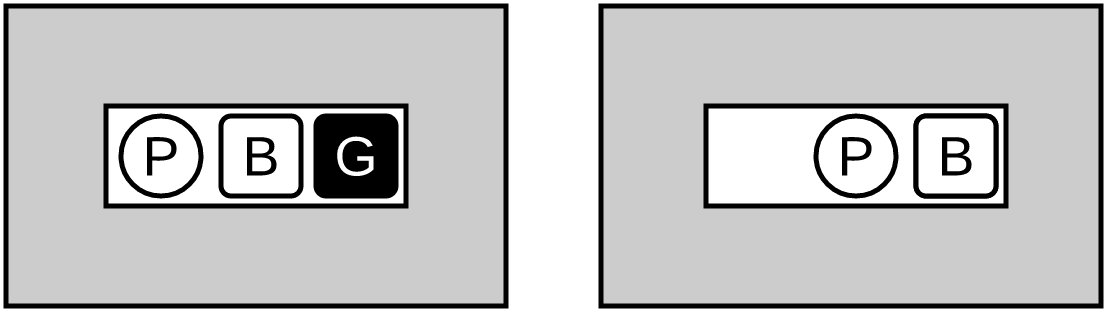
\includegraphics[width=0.7\linewidth]{images/basic_unsolved_solved.png}
  \caption{Simplest solvable Sokoban level.}
  \label{fig:b}
\end{figure}

The level depicted in figure \ref{fig:b} is the simplest solvable sokoban level that can be created. The solution to the puzzle is to simply move the player to the right one square. This action pushes the box onto the goal. Since there is only one box, and the box is covering a goal, the level is considered solved.

%--------------------------------------------------------------------------------
\SubSection{Rules}

The rules of the game are rather simple. During each turn, the player has the ability to move in one of four directions: up, down, left, or right. A square is considered empty if it does not contain a wall or box. If the square corresponding to the direction moved contains a box, and the next square is considered empty, the box is pushed into that square. This means the player can only push one box at a time. The player is allowed to move into any empty square. When every goal has been covered by a box, the puzzle is considered solved, and the game ends. Any box can be pushed onto any goal.  

%--------------------------------------------------------------------------------
\SubSection{Deadlock Detection}

Another important aspect of Sokoban is the existence of deadlocks. A deadlock is a configuration of objects that results in an unsolvable level [1]. A state is considered deadlocked if it contains at least one deadlock. Any action that the player takes has the potential of placing the level in a deadlocked state. If such a state is encountered, any attempt to solve the level should no longer be pursued, even if there are still valid actions that can be applied to the deadlocked state. While there are numerous types of deadlocks, two that are necessary for complete deadlock detection are simple deadlocks and freeze deadlocks. Implementation of the detection of these two deadlock types results in the ability to detect whether or not a action creates a deadlocked state. 

%--------------------------------------------------------------------------------
\SubSection{Simple Deadlocks}

Simple deadlocks are squares in the level that create a deadlock whenever a box is pushed into them. Pushing a block into a simple deadlock square creates a deadlock because the box in that square can no longer be pushed to a goal. These simple deadlock squares are independent of the positions of the boxes in the level, and do not change. This means that simple deadlock squares can be identified when the initial level is loaded. 

The algorithm for identifying simple deadlock squares is rather intuitive. By definition, if a box cannot be pushed from a square to one of the goals, the square is considered to be a simple deadlock square. Likewise, if a box cannot be pulled from one of the goals to that square, it means the same thing. This mean that all valid squares can be identified by removing all boxes from the level, placing a box on each goal square, pulling the box away in all directions, and marking all reachable squares as visited. Every square that is not marked as visited is a simple deadlock square. \cite{Wiki}

If we consider the level in figure \ref{fig:sd}, where the simple deadlock squares are crossed off, the algorithm becomes a little more clear. First we remove all boxes from the level. We then place an imaginary box on the goal and pull it in each direction. Since we cannot pull the box up, the space directly above the goal is a simple deadlock space. Since we cannot pull the box down, the square directly below the goal is a simple deadlock square. However, since we can pull the box to the left, the square directly to the left of the goal is considered a valid square. This square is then marked as visited, and we repeat the algorithm on this new square. 

\begin{figure}[h] 
  \centering
     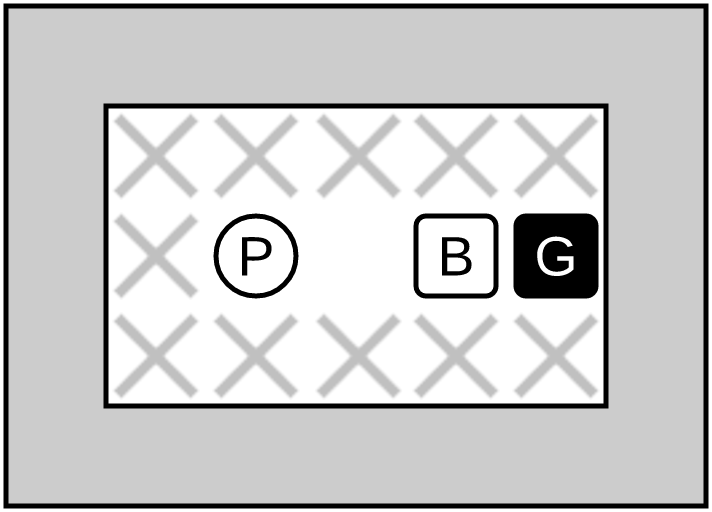
\includegraphics[width=0.5\linewidth]{images/simple_deadlock.png}
  \caption{Simple Deadlocks.}
  \label{fig:sd}
\end{figure}

The result of performing such an algorithm is the identification of all simple deadlock squares. When a box is moved, we can check the see if the square it is moved into is a simple deadlock square. If it is a simple deadlock square, we know there is a deadlock and the level can no longer be solved.

\begin{algorithm}
  \caption{Identifying simple deadlocks}
\begin{algorithmic}[1]
  \Function {IdentifySimpleDeadlocks}{}
    \State $stack\gets \textnormal{goals}$
    \State $visited\gets \emptyset$
    \While { stack not empty }
      \State $position\gets stack.pop()$
      \State visited.add(position)
      \For {direction = up, down, left, right}
        \If {can pull position in direction}
          \State $valid\gets \textnormal{move position in direction}$
          \State stack.add(position)
        \EndIf
      \EndFor
    \EndWhile
    \State \Return all squares - visited
  \EndFunction
  \end{algorithmic}
\end{algorithm}

%--------------------------------------------------------------------------------
\SubSection{Freeze Deadlocks}

Freeze deadlocks are configurations of boxes and walls that result in a deadlocked state. Unlike the simple deadlock squares, freeze deadlocks depend on the position of boxes in the level. This means that we must check for a freeze deadlock anytime a box is moved in the level. 

The level in figure \ref{fig:f} demonstrates an example of a freeze state. Notice how if either box is pushed up, it will be moved into a simple deadlock square. Since we can not push either box up, they are both blocked along the vertical axis. Since the blocks are side by side, any attempt to push the boxes left or right will fail. This mean each box is blocked along the vertical axis. Since both boxes are blocked along the vertical and horizontal axis, the entire configuration is considered a freeze deadlock, meaning no box in the configuration can be moved. However, if all boxes in the configuration are on goals, the level is considered to be in a semi-solved state, and there is no freeze deadlock. An example of such a configuration can be seen in figure \ref{fig:fok}.

\begin{figure}[h] 
  \centering
     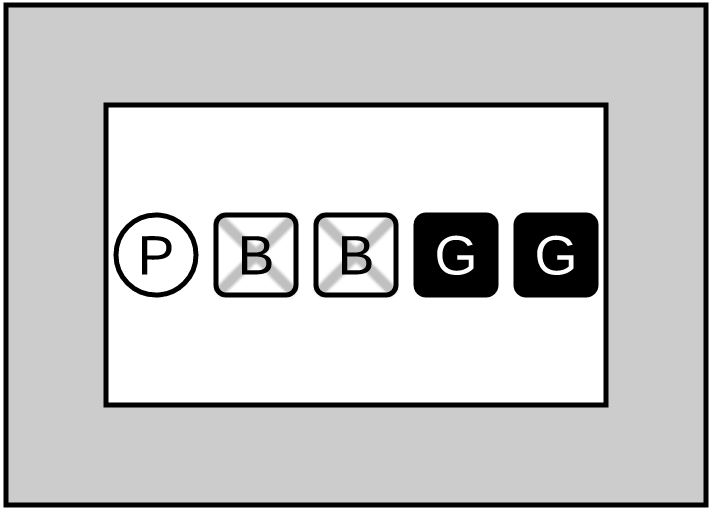
\includegraphics[width=0.5\linewidth]{images/freeze_deadlock.png}
  \caption{Freeze Deadlock.}
  \label{fig:f}
\end{figure}

\begin{figure}[h] 
  \centering
     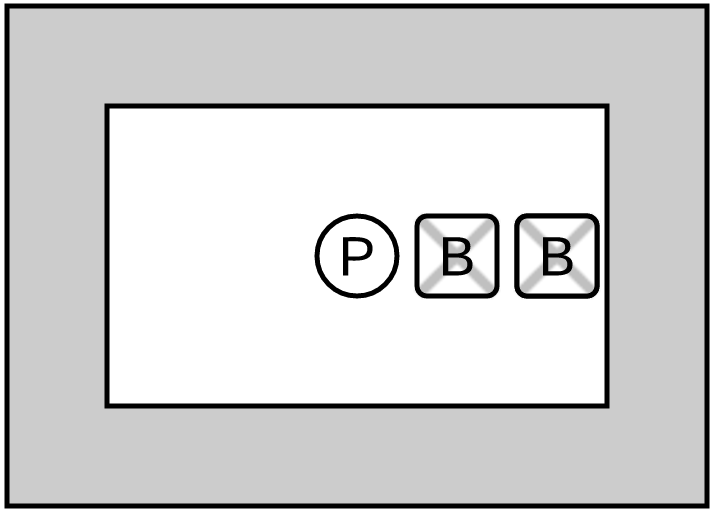
\includegraphics[width=0.5\linewidth]{images/freeze_deadlock_ok.png}
  \caption{Freeze Deadlock Exception.}
  \label{fig:fok}
\end{figure}

The algorithm for detecting freeze deadlocks is rather intuitive, since we only need to check whether a box can be pushed. Since a freeze deadlock is created after pushing a block, it is only necessary to check if the pushed box is frozen, and possibly the boxes around the pushed box. The following algorithm will identify whether or not pushing a box into a position will create a freeze deadlock. \cite{Wiki}

\begin{algorithm}
  \caption{Identifying freeze deadlocks}
\begin{algorithmic}[1]
  \State $frozen \gets \emptyset$
  \State $visited \gets \emptyset$
  \Function {Frozen}{position}
    \State $\textnormal{add position to visited}$
    \If { wall on left or right }
      \State $h\gets true$
    \ElsIf { simple deadlock on on left and right }
      \State $h\gets true$
    \ElsIf { box on left or right }
      \State $h\gets \textnormal{Frozen(left) or Frozen(right)}$
    \EndIf

    \If { wall on up or down }
      \State $v\gets true$
    \ElsIf { simple deadlock on on up and down }
      \State $v\gets true$
    \ElsIf { box on up or down }
      \State $v\gets \textnormal{Frozen(up) or Frozen(down)}$
    \EndIf
    \State \Return $\textnormal{h and v and all frozen on goals}$
  \EndFunction
  \end{algorithmic}
\end{algorithm}

%--------------------------------------------------------------------------------
\SubSection{Motivation}


Thought the research conducted within this paper outline and prove the application of Q-Learning as a solution to the Sokoban puzzle, it is also a case study into the possibility of using Q-Learning in problems relating to Sokoban, such as programming an autonomous robot to work in a warehouse. Such a robot would be required to navigate the warehouse, as well as perform its designated tasks, using only the information in its immediate vicinity.  It would be limited in the actions it can perform, and possibly in the knowledge it has of its environment. If such a robot’s task were to move crates into a storage location, then the two problems would be synonymous. In this case, a similar solution could be used to solve both problems. The data from our experiments are a proof that Q-Learning can be used to solve problems similar to Sokoban, and thus, has applications in the field of automation.  However, as the puzzles in Sokoban increase in difficulty, the time it takes to utilize our approach and find the optimal solutions increases as well.  So, although Q-Learning has applications in this field, it is unlikely that it will become the sole method of solving problems of this nature.

Another instance where the basic implementation of Q-Learning will fail is if there were more than a single agent acting within the environment. For example, imagine a situation where multiple autonomous robots are each moving boxes within a warehouse from location to location. If a basic Q-Learning approach were implemented, each robot would greatly increase the number of different states possible in the environment, and begin to interfere with one another.  In order to overcome this obstacle, a modification would need to be implemented such that the agent would be encouraged to communicate with one another.

%--------------------------------------------------------------------------------
\SubSection{Notation}

The state of a sokoban level can be encoded using a two dimensional arrangement of characters. Since there are really only eight possible permutations of objects in a Sokoban level, only eight characters are needed to completely encode the state. The characters shown in table \ref{table:notation} are commonly used among the Sokoban community to represent a sokoban level.

\begin{table}[htbp]
  \centering
  \begin{tabular}{l c} \hline\hline
    Square & Character \\ \hline
    Wall & \# \\
    Player & @ \\
    Player on goal & + \\
    Box & \$ \\
    Box on goal & * \\
    Goal & . \\
    Floor & Space \\ \hline\hline
  \end{tabular}
  \caption{The notation used to represent the state of a sokoban level.}
  \label{table:notation}
\end{table}

%--- Related Work ---------------------------------------------------------------
\Section{Related Work}

Previous implementations of solvers utilized graph search algorithms, such as Breadth-First and A*, to identify the optimal action policy. This is accomplished by constructing a graph of states where each state branches into four additional states. This branching is due to the fact that there are four possible actions that can be performed on each state. The goal of these graph search algorithms is to search for the state that takes the least number of action to create and is considered solved. Similar to the Q-Learning algorithm described in this paper, these graph search algorithms rely on an ability to reduce the search space through identification of deadlocks.

%--- Q-Learning -----------------------------------------------------------------
\Section{Q-Learning}

Q-Learning is a form of model-free reinforcement learning \cite{Watkins1992}. This techniques can be used to find the optimal action policy for any given markov decision process. A markov decision process is a mathematical framework used to model decision making problems where the decisions are under the agent's control. In Q-Learning, an agent experiences the following sequence of actions until the optimal action policy is identified. At any given state $s_t$ the agent can perform an action $a$. The result of taking action $a_t$ is the new state $s_{t+1}$. The agent recieved a immediate reward of $R_a(s_t, s_{t+1})$ for taking action $a_t$. Using this reward, the agent adjusts its $Q(s, a)$ values using the following equation \cite{Watkins1992}:

\begin{equation}
\label{eq:q}
\begin{split}
Q(s_t, a_t) \gets &Q(s_t, a_t) \\
                  &+ \alpha \cdot [R_a(s_t, s_{t+1}) \\
                  &+ \gamma \cdot \underset{a}{max}Q(s_{t+1}, a) - Q(s_t, a_t)]
\end{split}
\end{equation}

where 

\begin{equation}
\underset{a}{max}Q(s_{t+1}, a)
\end{equation}

is the maximum $Q(s, a)$ value that the agent can achieve from state $s_{t+1}$. This is determined by maximizing the $Q(s_{t+1}, a)$ value for every possible action that can be performed on state $s_{t+1}$. In the case of Sokoban, this means maximizing on the actions: up, down, left, and right. This results in the agent's ability to select actions that will produce the greatest reward. In a sense, the agent is maximizing the reward that they receive. 

In equation \ref{eq:q}, the learning rate is described using $\alpha \in (0, 1)$, and the discount factor is described using $\gamma \in (0, 1)$. The learning rate represents the rate at which the agent updates the $Q(s, a)$ values. When the learning rate is 0, the values will never change, meaning the agent will never learn. When the learning rate is 1, the agent will consider only the most recent information \cite{Littman94markovgames}. The discount factor controls the effect of future rewards in the decision making of the agent \cite{Littman94markovgames}. A discount factor of 0 will cause the agent to place emphasis on current rewards, and a discount factor of 1 will cause the agent to place emphasis on future rewards \cite{Littman94markovgames}. Our implementation utilizes a learning rate of 0.1 and a discount factor of 0.9. It is worth mentioning that the optimal learning rate and discount factor were not used in our implementation.

%--------------------------------------------------------------------------------
\SubSection{Rewards}

Rewards are one of the major building blocks of Q-Learning.  If you recall, a reward is given to an agent once an action $a_t$ is performed on a state $s_t$.  Many Q-Learning algorithms implement a reward function which, depending on the outcome state $s_{t+1}$, will result in a numerical reward.  These rewards will fall into one of two categories, negative or positive.  A positive reward should be given when a desirable outcome is achieved. The nature of the rewards implementation in the Q-Learning algorithm will cause the agent to prefer taking action $a_t$ at state $s_t$ again.  A negative reward should be given when an undesirable outcome.  Converse to the effect that the positive reward will have, the negative reward will cause the agent to avoid taking action $a_t$ at state $s_t$ again.  The formula for this reward is generally written as a difference function between the initial state $s_t$ and outcome state $s_{t+1}$ as seen in equation \ref{eq:reward}.

\begin{equation}
reward \gets R_a(s_t, s_{t+1})
\label{eq:reward}
\end{equation}

A list of the rewards given to our Sokoban agent for transitioning from state $s_t$ to outcome state $s_{t+1}$ can be seen in table \ref{table:rewards}.  We found that positive rewards should be given very rarely, and only in extremely desirable circumstances.  For instance, we gave the highest (positive) reward when a box was pushed onto a goal.  In the initial design of our solution, we gave the agent a reward of 0 for moving, because we saw no immediate negative or positive effects from this.  However, in our final implementation, we gave a negative reward to an agent for moving because this encouraged exploration, discouraged 'wondering', and prevented feedback loops.  A feedback loop occurs when the agent prefers a path which does not result in a solution, and prevents the agent from learning anything new.  For example, the agent would continuously push a box back and forth. The reason for this is because both moving and pushing a box provided positive rewards to the agent. 

In the development of a successful Q-Learning algorithm, we found the adjustment of the rewards to provide the most significant impact on the success rate of the solver.

\begin{table}[htbp]
  \centering
  \begin{tabular}{l c} \hline\hline
    Transition & Reward \\ \hline
    Box pushed onto goal & $+1.00$ \\
    Box pushed & $-0.01$ \\
    Agent moved & $-0.15$ \\
    Box pushed against wall & $-0.15$ \\
    Box pushed against box & $-0.15$ \\
    Box pushed from one goal to another & $-0.15$ \\
    Box pushed off goal & $-0.20$ \\ 
    Agent moved into wall & $-1.00$ \\
    Agent moved into immovable box & $-1.00$ \\
    Agent created simple deadlock & $-1.00$ \\
    Agent created freeze deadlock & $-1.00$ \\ \hline\hline
  \end{tabular}
  \caption{Immediate rewards for transitioning a Sokoban level.}
  \label{table:rewards}
\end{table}

%--------------------------------------------------------------------------------
\SubSection{Implementation}

Algorithm \ref{alg:q_learning} represents the entry point for the Sokoban solver.  An initial state $s_0$ and desired episodes will be used to run an iterative learning process on the state.  An episode represents one iteration of learning from initial state to terminal state.  A larger number of episodes run during Q-Learning will result in a more optimal solution.

\begin{algorithm}
  \caption{Solver for Sokoban using Q-learning}
  \begin{algorithmic}[1]
    \Function {QLearning}{state, episodes}
      \State $Q\gets \emptyset$
      \State $episode\gets 0$
      \While {$episode\not=episodes$}
        \State $Q\gets \Call{RunEpisode}{Q}$
        \State $episode\gets episode + 1$
      \EndWhile
      \State \Return Q
    \EndFunction
  \end{algorithmic}
\label{alg:q_learning}
\end{algorithm}

Algorithm \ref{alg:run_episode} \cite{Russell}\cite{Guo} is where the majority of the Q-Learning is completed, and is used to determine the optimal strategy for solving a given Sokoban puzzle.  We run an episode of Q-Learning on an initial state with persistent Q values.  While state $s_t$ is not terminal, we pick an action which will maximize the Q value that can be reach, since this is by definition the highest rewarded action that the agent can take at $s_t$.  Once we take action $a_t$, we calculate the outcome state $s_{t+1}$ and update the Q value for $s_t$ taking action $a_t$.  This update of the Q value is effectively causing the agent to learn based on the action that is taken.

\begin{algorithm}
  \caption{Runs a single episode of Q-learning}
  \begin{algorithmic}[1]
    \Function {RunEpisode}{state, Q}
      \State $state\gets \textnormal{initial state}$
      \State $\alpha \gets 0.1$ \Comment{Learning Rate}
      \State $\gamma \gets 0.9$ \Comment{Discount Factor}
      \While {not state.Terminal?}
        \State $action\gets \Call{MaximizeAction}{state, Q}$
        \State $resultState\gets \Call{TakeAction}{state, action}$
        \State $maxQ\gets \Call{MaximizeQ}{state, Q}$
        \State \begin{varwidth}[t]{\linewidth}
          $Q(state, action) \gets Q(state, action) +$\par
          \hskip\algorithmicindent $\alpha \cdot [R(state, resultState) +$\par
          \hskip\algorithmicindent $\gamma \cdot maxQ - Q(state, action)]$
        \end{varwidth}
      \EndWhile
      \State \Return Q
    \EndFunction
  \end{algorithmic}
  \label{alg:run_episode}
\end{algorithm}

Algorithm \ref{alg:maximize_q} is used to calculate the maximum Q value that can be reached in a single action $a_t$ from state $s_t$.  A simple iteration over the actions possible at that state will yield the maximum Q value.  Similarly, Algorithm \ref{alg:maximize_action} is used to find the action which will yield the maximum Q value.  If many action will result in an equal Q value, we randomly pick one.  In the sokoban puzzle, these two algorithms are the main logic for the agent to use its learned knowledge to perform actions resulting in the highest possible reward.  Since the sokoban agent can take only one of four possible actions - up, down, left, and right - they must look at each of these and make an informed decision to which will produce the highest reward.  If there are more than one action that produces the highest value, the agent will select a random action from that set.

\begin{algorithm}
  \caption{Returns the maximum Q value reachable from a state in a single action}
  \begin{algorithmic}[4]
    \Function {MaximizeQ}{state, Q}
      \State $max\gets -\infty$
      \For {$ action \in \left\{ {up, down, left, right}\right\}$}
        \If {$Q(state, action) > max$}
          \State $max\gets Q(state, action)$
        \EndIf
      \EndFor
      \State \Return $max$
    \EndFunction
  \end{algorithmic}
  \label{alg:maximize_q}
\end{algorithm}

\begin{algorithm}
  \caption{Returns the action which will achieve the maximum q value reachable from a state}
  \begin{algorithmic}[1]
    \Function {MaximizeAction}{state, Q}
      \State $max\gets -\infty$
      \State $actions\gets \emptyset$
      \For {$ action \in \left\{ {up, down, left, right}\right\}$}
        \If {$Q(state, action) > max$}
          \State $max\gets Q(state, action)$
          \State $actions\gets \left\{ {action}\right\}$
        \Else
          \State $actions \gets actions \cup \left\{ {action}\right\}$
        \EndIf
      \EndFor
      \State \Return random action from $actions$
    \EndFunction
  \end{algorithmic}
  \label{alg:maximize_action}
\end{algorithm}

Algorithm \ref{alg:take_action} is used to perform action $a_t$ on state $s_t$ which will produce an outcome state $s_{t+1}$.  Because this is highly dependent on the implementation your Sokoban puzzle, this has been left, for the most part, unimplemented.  In our final implementation of the Sokoban solver, we incorporated our reward function into this algorithm.  When action $a_t$ is performed on state $s_t$ it produces an outcome state $s_{t+1}$ as well as returning an appropriate reward for the transition.

\begin{algorithm}
  \caption{Returns the resulting state after an action is taken on an initial state}
  \begin{algorithmic}[1]
    \Function {TakeAction}{state, action}
      \State \Return state after action is taken
    \EndFunction
  \end{algorithmic}
  \label{alg:take_action}
\end{algorithm}

%--- Experimental Analysis ------------------------------------------------------
\Section{Experimental Analysis}

In order to evaluate the performance of our solver, we selected three levels with various difficulty. The levels were classified into three groups, easy, medium, and hard. These difficulties are based on the minimum number of moves required to solve the puzzle, and the number of boxes in the puzzle. In order to understand the exact capabilities of the solver, the following parameters were measured after each episode: the number of moves the agent takes, the average reward the agent received, whether or not the agent was able to solve the puzzle, and the time it took for the agent to complete the episode. 

\begin{table}[htbp]
  \centering
  \begin{tabular}{l c c c} \hline\hline
    Difficulty & Boxes & Moves & Episodes \\ \hline
    Easy & 1 & 11 & 70 \\
    Medium & 2 & 9 & 140 \\
    Hard & 2 & 30 & 400 \\ \hline\hline
  \end{tabular}
  \caption{Results from solving 3 different puzzles.}
  \label{table:results}
\end{table}

\begin{figure}[h] 
  \centering
     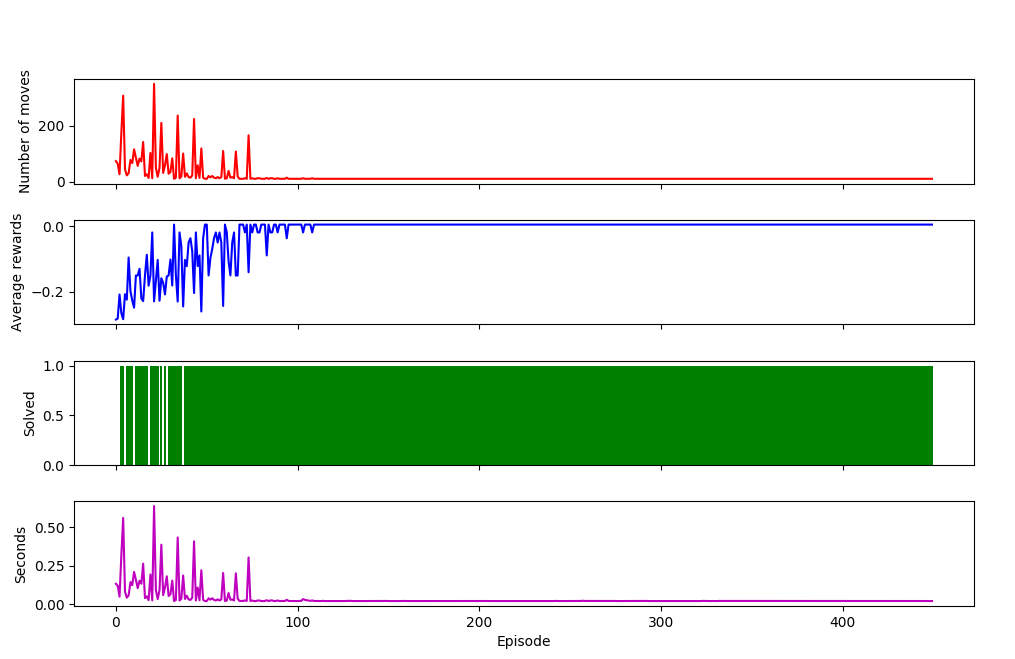
\includegraphics[width=\linewidth]{images/easy_graph.png}
  \caption{Results for solving an easy level.}
  \label{fig:e}
\end{figure}

The results from figure \ref{fig:e} demonstrate the solver's ability to identify the optimal action policy after only 100 episodes. Although the number of moves the solver used to solve the puzzle stabilized at 11 after only 70 episodes, the average reward for each episode did not stabilize until episode 100. Instead, the average reward continued to increase until its maximum at episode 100. This demonstrates the ability of the solver to refine the action policy through continuous exploration. Although the agent identified an action policy that would solve the puzzle, they continued to search for an even better action policy. However, since no better action policy was found, the agent continued to use the action policy that they knew would produce the greatest reward.

\begin{figure}[h] 
  \centering
     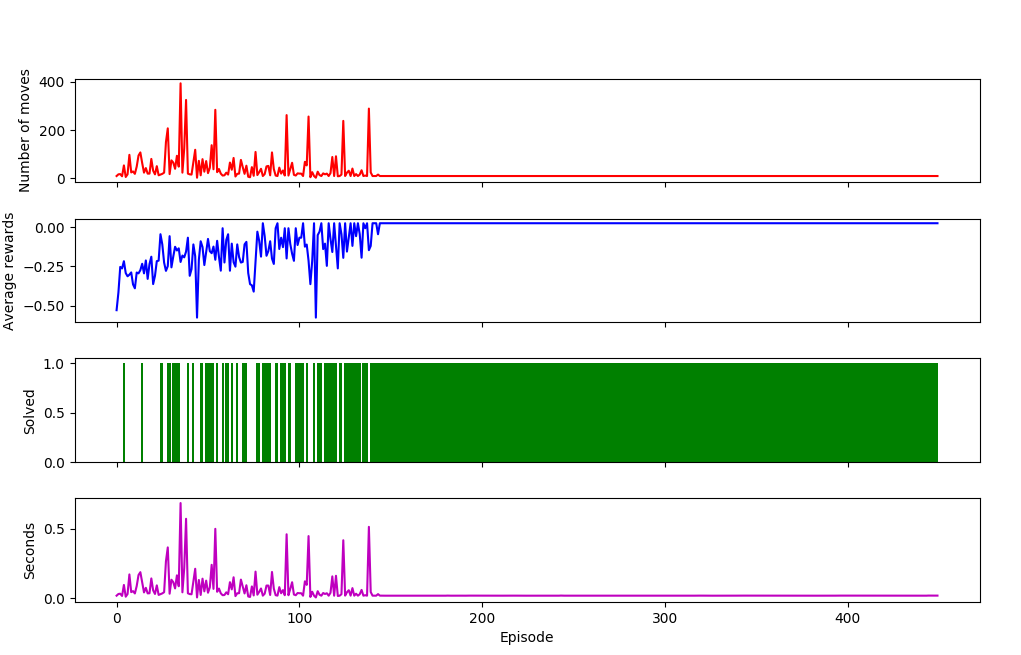
\includegraphics[width=\linewidth]{images/medium_graph.png}
  \caption{Results for solving an medium level.}
  \label{fig:m}
\end{figure}

The level that produced the results in figure \ref{fig:m} was a bit more challenging than the level that produced the results to figure \ref{fig:e}. Though the number of moves required to solve the level was only 9, compared to the 11 moves required to solve the other level, the number of boxes increased to two. This increases the complexity of the level greatly. After about 140 episode, the solver was able to identify the optimal action policy.  

\begin{figure}[h] 
  \centering
     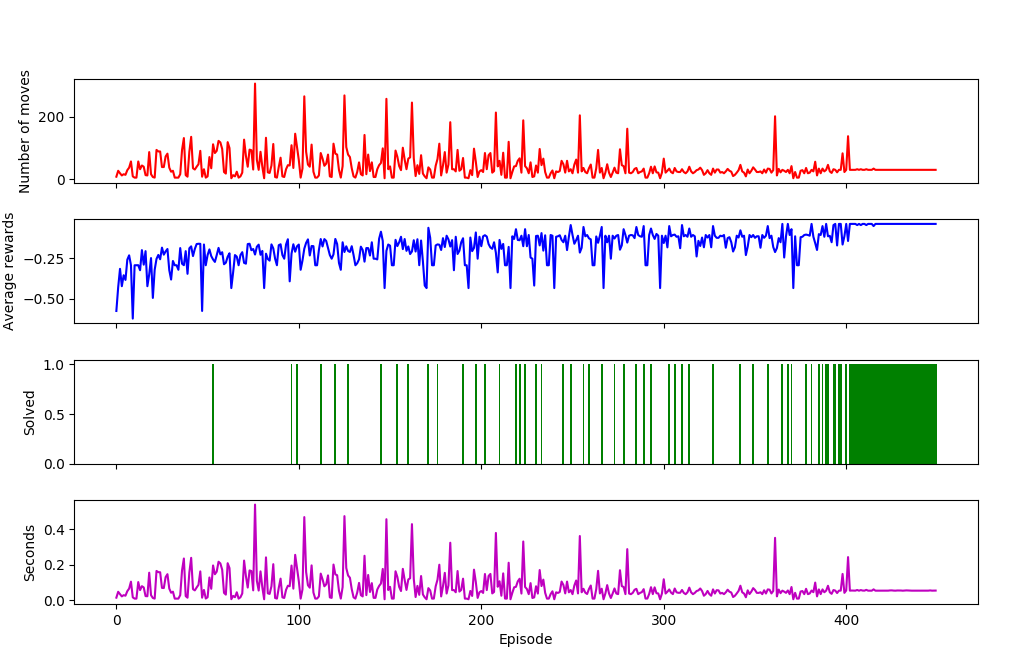
\includegraphics[width=\linewidth]{images/hard_graph.png}
  \caption{Results for solving an hard level.}
  \label{fig:h}
\end{figure}

The level that produced the results in figure \ref{fig:h} takes a minimum of 30 moves to solve and contained two boxes, making it the most complicated level that was tested. The solver was able to identify the optimal action policy after about 400 episodes. The results from this data provided the most insight into the solvers performance. The number of moves that the solver used began small, increasing until about episode 80, then decreasing until about episode 400. If the solvers goal is to minimize the number of moves, why was the number of moves increasing? Though the number of moves was increasing, the agent was not solving the level. instead, the agent was creating deadlocks and the episode was ending early. This allowed the agent to identify the actions that created deadlocks and increase the number of moves they were able to take. When all deadlocks were identified, after approximately 80 episodes, the agent could then refine the action policy and reduce the overall moves they needed to take.

%--- Future Works ----------------------------------------------------------------
\Section{Future Works}

In future implementations of this experiment, it will be fundamental that different combinations of learning rate and discount factor are tested, analysing the correlation it has on the solver.  Within the experiment that was conducted, we selected the learning rate and discount factor based on the immediate correlation that was seen with the success rate of the solver; by no means, however, are these values ($learning rate \gets 0.20$, $discount factor \gets 0.80$) the most optimal.  Moreover, an experiment using a dynamic learning rate and discount factor should be performed, determining if it has any correlation with the success rate or speed of the solver.  We theorize that if we begin with a higher learning rate and, throughout the learning process, gradually diminish the rate, it would have a strong effect on the success rate of the solver, modeling that of a human and our learning process.

Also, we would like to experiment with different types of reward functions.  In the experiment that was conducted, static rewards were assigned to each type of scenario that could occur during the puzzle.  We would like to apply a reward function for certain scenarios that is dependent on the overall progress towards success on the state.  For example, when the agent pushes a box onto a goal, the reward that is received would be dependent on how many goals are already covered, as opposed to a static value of $+1.00$.  We believe that it is worth testing if this strategy has any effect on the success and speed of the solver.

It would also be worth testing various graph search algorithms used to solve Sokoban puzzles, such as A* and A* Iterative Deepening, in order to compare and contrast the effectiveness of these algorithms to that of Q-Learning.

%--- Conclusions ----------------------------------------------------------------
\Section{Conclusions}

%--- Appendix ----------------------------------------------------------------
\appendix
\listoffigures
\listoftables

%--- Bibliography ---------------------------------------------------------------
\bibliographystyle{latex8}
\bibliography{latex8}

\end{document}


